% !TEX root =  ../main.tex
\section{Computing a guide path in $C_{reach}$ ($\mathcal{P}_1$) }
\label{rbprm}

We consider the issue of computing a normalized guide path $\mathbf{q}^0(t) : [0,1] \longrightarrow \mathbb{R}^r$ for the root of a multiped robot, connecting user-defined start and goal configurations. As said in the previous section, the goal is to enforce that the guide can be discretized into a sequence of \gls{contact feasible} configurations. We denote by \gls{ccontact} the contact sub-manifold of the robot.

We say that a root configuration $\mathbf{q}^{0}$ is \gls{contact feasible} if it belongs to the set:
\begin{equation}
      C_{contact}^0= \{ \mathbf{q}^{0}: \exists \mathbf{q}^{\overline{0}}, \mathbf{q}^{0} \oplus \mathbf{q}^{\overline{0}} \in C_{contact} \}
    \label{eq:pi}
\end{equation}

%~ The set of all \textit{geometrically feasible} root configurations is denoted by $C_{reach}$.
By extension, a path $\mathbf{q}^0(t)$ is \gls{contact feasible} if $\forall t \in [0,1], \mathbf{q}^0(t) \in C_{contact}^0$.

For this stage, and for this stage only, we make the assumption that for \gls{cluttered} problems, a \gls{contact feasible} path can be transformed into a \gls{equilibrium feasible} path.
Under this assumption, for a two-stage acyclic contact planner to be exact and complete, we need the combination of two conditions on a guide path generator: all the generated paths must be \gls{contact feasible} (sufficient condition); the guide planner must be complete, i.e. it must be able to discover any \textit{contact feasible} path (necessary condition).

In this Section we characterize \gls{ccontact0} theoretically with a necessary and a sufficient condition for belonging to the set.
We then approximate \gls{ccontact0} as a space $C_{reach}$, where we can efficiently sample configurations.
We finally describe our implementation of an efficient RRT planner in $C_{reach}$.

   
%~ We want all the configurations of $q^0(t)$ to belong to a set $C_{reach}$ defined as:
%~ 
%~ \begin{eqnarray}
%~ C_{reach}= \{ \mathbf{q}^{0} & : & \exists f, f(\mathbf{q}^{0}) \in C_{contact} \}
%~ \end{eqnarray}
 
\subsection{Conditions for contact feasibility}
By default, \glslink{contact feasible}{\textit{contact feasibility}} implies a constructive demonstration by exhibiting a valid $\mathbf{q}^{\overline{0}}$. This is the approach chosen by \cite{Bouyarmane2009}. However, computing $\mathbf{q}^{\overline{0}}$ is expensive in terms of computation time. In this section we rather define a necessary condition and a sufficient condition for \glslink{contact feasible}{\textit{contact feasibility}} that do not require this explicit computation.




\subsubsection*{Contact feasibility: necessary condition}
For a contact to be possible, a volume $O_i \in O$ necessarily intersects with the reachable workspace $W(\mathbf{q}^{0})$ (Figure~\ref{fig:contact_gen}--1). Furthermore, if $\mathbf{q}^{0}$ is  feasible, then the trunk of the robot $W^0(\mathbf{q}^{0})$ is necessarily not colliding  with the environment $O$.

Therefore we can define an optimistic approximation  $C^0_{Nec} \supset$ \gls{ccontact0} defined as: 
\begin{equation}
C_{Nec}^0 = \{ \mathbf{q}^0 : W(\mathbf{q}^{0}) \cap O \neq \emptyset \text{ and } W^0(\mathbf{q}^{0}) \cap O = \emptyset \} % \\ }
 %~ & \wedge & A_{trunk}(\mathbf{q}^{root}) \cap W = \emptyset \}
\end{equation}
The inclusion \gls{ccontact0} $\subset C^0_{Nec}$ is straightforward, but it is very important.
Planning in $C^0_{Nec}$ allows a strong reduction of the search space, while not discarding 
any root configuration that could lead to a solution.
 
The condition defining $C^0_{Nec}$ is only necessary. This means that it might not be possible to extend a guide path planned 
in $C^0_{Nec}$ into a sequence of contact configurations.

\subsubsection*{Contact feasibility: sufficient condition}
%~ In building $C_{reach}^1$, we directly considered the including hull of the root body $W^{0}$, obtaining a necessary condition. 
A trivial sufficient condition for \glslink{contact feasible}{\textit{contact feasibility}} can be constructed as a variation of $C^0_{Nec}$, by replacing $W^0$ with a bounding volume $B^{Suf}$ encompassing the whole robot in a given pose, except for the effector surfaces to be in contact. We denote by \mbox{$C_{Suf}^0 \supset $ \gls{ccontact0}} the set of root configurations corresponding to this sufficient condition.

In general, the inclusion is strict, which means that we lose the completeness of the two-stage contact planner (i.e. the planner is not able to discover a path inside \mbox{$C_{reach} \setminus C_{Suf}^0$}). However, the sufficient condition guarantees that any such path leads to a valid sequence of contacts.

\subsection{Contact feasibility: a compromise \gls{reachc}}
The sufficient condition is not interesting in practice since it leads the solver to lose too many interesting paths. The necessary condition is not perfect either, since the first stage of the planner would stop on a guide that is not \gls{contact feasible} in practice. It might be possible to find an ideal shape $B$ that is necessary and sufficient; however, it seems intuitively very unlikely in general. The construction of a shape $W^0 \subset B \subset B^{Suf}$ leading to a necessary and sufficient condition (or the proof of its nonexistence) is out of the scope of this work.

However, between $W^0$ and $B^{Suf}$, a trade-off can be found between a necessary and a sufficient condition. We define $W^0_s$ as the volume $W^0$ subject to a scaling transformation by a factor $s \in \mathbb{R}^+$.
%
We then consider the spaces $C_{s}^0$
 \begin{equation}
C^0_s = \{ \mathbf{q}^0 : W(\mathbf{q}^{0}) \cap O \neq \emptyset \wedge W^0_s(\mathbf{q}^{0}) \cap O = \emptyset \} % \\ }
 %~ & \text{ and } & A_{trunk}(\mathbf{q}^{root}) \cap W = \emptyset \}
\end{equation}
%
If $s=1$, then $W^0_s$ = $W^0$, such that $C_1^0$ = $C_{Nec}$. We thus define $s \in \mathbb{R}^+$, since values inferior to $1$ can only introduce more errors.
The higher $s$, the closer this \gls{reachc} is to being sufficient, and if $s=1$, the search is complete (in the sense that all \gls{contact feasible} configurations can be found). The parametrization of $s$ defines a trade-off between these two desirable properties. $s$ can be chosen by hand, or automatically as explained in Section~\ref{sec:params}.
In the rest of the paper, we consider that an appropriate value $s^*$ of $s$ is chosen, and define \gls{creach0} $= C^0_{s^*}$.

As an example, Figure~\ref{fig:HyQ_roms} presents the volumes $W$ computed for the HyQ robot.
In Appendix~\ref{app:rom}, we give a generic method to compute these volumes, with the example of HRP-2.
%~ Section~\ref{sec:results} shows that in practice, it is easy to adjust $s$ to keep most of the interesting guides without introducing incorrect guides.

\begin{figure}
  \centering
  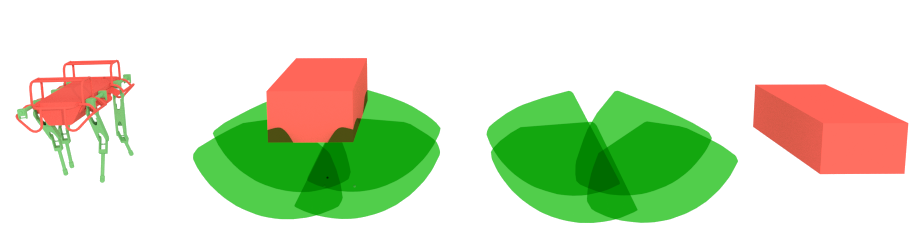
\includegraphics[width=0.95\linewidth]{figures/HyQ_roms}
  \caption{
           $W$ volumes for HyQ. The green shapes represent the reachable workspace $W^k$ of each limb. The red shape is $W^0$, a scaling of the convex hull
           of the torso of the robot.}
		   \label{fig:HyQ_roms}
\end{figure}

\subsection{Computing the guide path in $C_{reach}^0$}
Any sampling-based motion planner can be used to plan a path in \gls{creach0}. 
Indeed, contrary to \gls{ccontact}, \gls{creach0} has a non zero measure in the configuration space $C$. Therefore a standard uniform sampling approach
can work, in spite of a high rejection rate. 
Thus, the only significant change regarding a classical planner is to replace the classical collision checking method with a test of belonging to \gls{creach0} when verifying
that drawn configurations and associated local paths are valid.

However, to improve the sampling efficiency while remaining probabilistically complete, we bias the sampling process to generate near obstacle configurations, similarly to~\cite{Amato98choosinggood}.
First, a configuration is set to a random point on the surface of one randomly chosen obstacle. The root location is then translated and rotated randomly until the \gls{reachc} is satisfied.
Our current implementation of these modifications is based on the Bi-RRT planner \citep{770022} provided by the HPP software.

Thanks to this set of modifications, the problem of planning an \gls{contact feasible} path in a high dimensional space is reduced to a standard geometry and collision checking problem, in a much lower dimension (6 for HyQ, 8 for HRP-2 that has joints in the torso). In so doing we make the problem tractable for sampling-based approaches, with \gls{interactive} computation times.
